\documentclass[12pt]{article}

\usepackage{sbc-template}

\usepackage{graphicx,url}

\usepackage[T1]{fontenc}
\usepackage[brazilian,portuges]{babel}
\usepackage[utf8]{inputenc}

\sloppy

\title{A Systematic Mapping Study on Quality of Service in Service-Oriented Computing}
\author{Danilo Filgueira Mendon\c{c}a\inst{1}, Gena\'{i}na Nunes Rodrigues\inst{1}, \\ Rodrigo Bonif\'{a}cio\inst{1}, Alet\'{e}ia Favacho\inst{1}, Maristela Holanda\inst{1} }

\address{Department of Computer Science -- University of Brasilia (UnB) -- Campus Darcy Ribeiro\\
70910-900, Brasilia, DF, Brazil
\email{dfmendonca@gmail.com, \{genaina, rbonifacio, aleteia, mholanda\}@cic.unb.br}
}

\begin{document} 

\maketitle

\begin{abstract}
  In the last years, the field of service oriented computing (SOC) has received a growing interest from researchers and practitioners, particularly with respect to quality of service (QoS). This paper presents a mapping study to aggregate literature in this field in order to find trends and research opportunities in the regarding QoS in SOC. We analysed 250 papers and we were able to identify major groups that have contributed to different aspects in the context of our study. We also show that, with respect to SOC contributions dealing with QoS properties, most of them concentrate on runtime issues, such as monitoring and adaptation. Regarding quality attributes, a vast majority the papers use generic models, so that the proposed solutions are independent of the particularities of a quality attribute. In spite of that, we find that availability and performance were the major highlights. With respect to research type, most of the reviewed studies propose new solutions, instead of evaluating and validating existing proposals--- a symptom of a field that does not follow established research paradigms.
\end{abstract}

\begin{resumo}
  Nos últimos anos, o campo da computação orientada a serviços (SOC) recebeu um crescente interesse de pesquisadores e praticantes, particularmente no que diz respeito a qualidade de serviços (QoS). Esse artigo apresenta um estudo de mapeamento para agrupar a literatura neste campo. Nossas maiores descobertas mostram que, em relação às contribuições para SOC envolvendo propriedades de QoS, a maioria se concentra em monitoramento e adaptação, enquanto poucas focam em coordenação e comunicação. A respeito dos atributos de qualidade, uma vasta maioria dos artigos utilizam modelos genéricos, de modo que suas contribuições são independentes das particularidades de um dado atributo. Não obstante, descobrimos que disponibilidade e desempenho foram os principais destaques, ao contrário de custo, escalabilidade e segurança. A respeito do tipo de pesquisa, a maioria dos estudos avalizados propuseram novas soluções em vez de avaliarem ou validarem propostas existentes --- um sintoma de um campo que não segue paradigmas de pesquisa estabelecidos.
\end{resumo}

\newcommand{\AllPubs}{1034 }
\newcommand{\AcceptedPubs}{249 }
\newcommand{\CoodenacaoComunicacao}{9.64\%}
\newcommand{\Ciclodevida}{14.46\%}
\newcommand{\Composicao}{27.31\%}
\newcommand{\DescobrimentoSelecao}{28.11\%}
\newcommand{\ModelosdeQoSeLinguagens}{33.73\%}
\newcommand{\MonitoramentoAdaptacao}{34.94\%}
\newcommand{\Seguranca}{10.84\%}
\newcommand{\Custo}{12.45\%}
\newcommand{\Confiabilidade}{26.51\%}
\newcommand{\Disponibilidade}{30.92\%}
\newcommand{\Desempenho}{38.15\%}
\newcommand{\SLA}{58.63\%}
\newcommand{\Outros}{6.83\%}
\newcommand{\Escalabilidade}{6.83\%}
\newcommand{\Pessoal}{0.40\%}
\newcommand{\Validacao}{19.28\%}
\newcommand{\Avaliacao}{45.78\%}
\newcommand{\Solucao}{92.77\%}


%TCIDATA{LaTeXparent=0 0 sbrc_2013.tex}
%Introdução

\section{Introdu\c{c}\~{a}o}\label{sec:introduction}

SOC, SOA, \textit{Web Services}, SOAP, REST, Orientação a Serviços, Computação em Nuvem. Nos últimos anos esses e outros acrônimos tornaram-se frequentes na tecnologia da informação. O surgimento de um novo paradigma, impulsionado pelo amadurecimento da internet e pela proximidade crescente entre negócios e TI, criou novos caminhos e oportunidades para trabalhos de desenvolvimento e pesquisa. Nesse sentido, um grande número de estudos foram e vem sendo conduzidos com foco nos diversos aspectos da computação orientada a serviços, tais quais arquitetura, modelos, métodos, processos, ferramentas diversas, frameworks, métricas, problemas solucionados e ainda vigentes. Desta forma, a intenção daqueles interessados em iniciar suas atividades na área fica comprometida pela dificuldade em se obter informações claras sobre o atual estado da arte, os desafios e os temas mais abordados e aqueles com deficit de pesquisas. Esses dados são cruciais para que esforços sejam bem direcionados e para que a ciência caminhe em cooperação e com eficiência.

Um mapeamento sistemático de estudos visa classificar de forma sistemática e ampla um conjunto de estudos. Dada a grande quantidade de publicações no escopo da orientação a serviços, sua metodologia ágil e que permite a análise de um maior número de estudos justifica sua escolha em detrimento de outras metodologias, como o \textit{Systematic Literature Review} \cite{Petersen_Feldt_Mujtaba_Mattsson_2007}. Essa última exige uma análise minuciosa e detalhada de cada publicação, o que requer um esforço considerável e inviabiliza a inclusão de um grande número de publicações num quadro de poucos pesquisadores. Assim, dados os fatos citados e o interesse em se obter uma classificação ampla e significativa da ciência relacionada à orientação a serviços, de caráter inicial e que irá servir de subsídio a outros estudos, este trabalho de conclusão de curso em Engenharia de Redes de Comunicação realiza um mapeamento sistemático de estudos abrangendo a orientação a serviços. 

Segundo \cite{Papazoglou:2007:SOA:1265289.1265298}, devido ao crescente acordo na implementação e gerência de aspectos funcionais de serviços, tal qual a adoção de WSDL para a descrição, SOAP para troca de mensagens, ou WS-BPEL para a composição, os interesses de pesquisadores estão se voltando aos aspectos não funcionais de aplicações orientadas a serviços. Visando essa constatação, nosso mapeamento irá concentrar-se na questão de qualidade, ou aspectos não funcionais, sobretudo a qualidade de serviços, termo aqui empregado de forma literal e posterior ao termo QoS, uma vez que os principais agentes do paradigma em questão são, coincidentemente, denominados serviços. Ademais, o ambiente proposto pelo SOC está sujeito a condições particulares diferentes daquelas já estudadas e conhecidas em outros paradigmas, havendo variáveis que elevam a complexidade da análise de parâmetros de qualidade, tanto na fase de planejamento quanto em fase de execução por meio do monitoramento e da gerência dos serviços, sendo esse um obstáculo sólido à adoção de arquiteturas como o SOA. Nesse sentido, o presente estudo visa mapear as publicações relacionadas a essas questões, contemplando cenários com ou sem o uso de SOA, proporcionando uma redução da incerteza quanto ao atual estado de desenvolvimento da ciência contribuinte ao tema abordado e quanto aos desafios e avanços já conquistados.

No que tange a trabalhos relacionados, este trabalho possui características inéditas dentro do campo de QoS em SOC. Dentre as referências atuais e mais relevantes no que concerne modelos de QoS em SOC pode ser encontrado em \cite{pernici}, produzido pelo projeto europeu S-CUBE~\cite{scube}. Esta, além desse citado, produziu uma coletânea de outros relatórios e trabalhos que analisam publicações em praticamente todas as eferas do SOC. Entretanto, trata-se de trabalhos de Systematic Literature Review, visto que analisam profundamente as publicações envolvidas na área e as restringe àquelas com maior qualidade e aceitação, indicando as vantagens e limitações das propostas analisadas. Em contraste, o MS proposto abrange um número maior de estudos, trazendo informações em categorias mais amplas e que possibilitam a melhor análise geral da pesquisa relacionada. São dados amplos mas sensíveis para a compreensão do estado da ciência envolvida com os aspectos qualitativos do SOC.

Em geral, o resultado de um estudo de mapeamento é um mapa visual classificando os resultados obtidos. Em particular, acreditamos que esse mapeamento pode beneficiar o estado da arte e da pr\'{a}tica em Computa\c{c}\~{a}o Orientada a Servi\c{c}os identificando tend\^{e}ncias e oportunidades para transfer\^{e}ncia de conhecimento. Considerando tamb\'{e}m o tamanho e abrang\^{e}ncia dessa \'{a}rea outros  objetivos do presente mapeamento de estudos s\~{a}o tamb\'{e}m esclarecer o paradigma da orientação a serviços no contexto de qualidade de servi\c{c}os (QoS) por meio de uma classificação ampla e sistemática, obtendo informações sobre frequências de publica\c{c}\~{o}es, \'{a}reas e t\'{o}picos de pesquisa, enfoques, tipos de contribui\c{c}\~{o}es de pesquisa dadas, os agentes e f\'{o}runs envolvidos.

As demais se\c{c}\~{o}es desse artigo est\~{a}o organizadas da seguinte forma: Se\c{c}\~{a}o \ref{?}.Se\c{c}\~{a}o \ref{?}. Se\c{c}\~{a}o \ref{?}. Finalmente, na Se\c{c}\~{a}o \ref{?} apresentamos um resumo das nossas descobertas e provemos tamb\'{e}m algumas discuss\~{o}es finais. 

%Neste mapeamento, deve-se prezar pelo uso de ferramentas de apoio e que agilizem os procedimentos sistemáticos a serem seguidos. Não é seu objetivo avaliar qualitativamente os trabalhos de pesquisa classificados, mantendo a análise a um nível menos detalhado e que permitirá a inclusão dessas publicações em categorias abrangentes e significativas e que não exijam a minuciosa análise de cada uma delas. 

%Em relação aos atributos de QoS, tem-se por objetivo compreender que tipo de intervenções vem sendo feitas para a absorção de aspectos de qualidade em SOC e sua melhoria, identificando quais tipos de pesquisa,  de contribuição e quais atributos ou contextos tem maior importância, quais representam os maiores desafios para a concretização da adoção deste paradigma e quais são pouco abordados. Entre os variados e numerosos tipos de atributos que atendem a diversos modelos, este trabalho visa aqueles cuja definição encontra-se bem difundida e aceita entre os trabalhos relacionados. São eles o desempenho, a disponibilidade, a confiabilidade, a segurança, a modificabilidade, a testabilidade, a escalabilidade, o custo e outros para que os demais atributos sejam representados agrupadamente. Entre os tipos de pesquisa aceitos, estão os de avaliação, solução, validação, filosófico e de experiência pessoal. Por fim, entre os tipos de contribuições dadas, estão as de modelo, método, processo, ferramenta e métricas.

    
%TCIDATA{LaTeXparent=0 0 sbrc_2013.tex}
%Review Method

\section{Método do Estudo}\label{sec:review_method}

Um mapeamento sistemático tem por objetivo classificar informações acerca de uma área de pesquisa de forma ampla e menos minuciosa que a tradicional revisão sistemática de estudos. Uma vez constatada a vasta quantidade de publicações no campo de SOC, escolheu-se esta metodologia para viabilizar a classifica\c c\~{a}o dos artigos. A metodologia adotada seguiu as diretrizes propostas em \cite{petersen:sms2008}, cujos passos necess\'{a}rios s\~{a}o descritos no restante desta se\c c\~{a}o.

\subsection{Protocolo do Estudo}

Um MS, assim como outras revisões literárias, estabelece o uso de um protocolo que documenta as etapas do mapeamento de modo a garantir sua replicação e diminuir possíveis erros por parte dos pesquisadores. Nele estão definidas as questões de pesquisa, os fóruns científicos onde as publicações s\~{a}o recuperadas, a \textit{string} de busca utilizada, os critérios de inclusão e exclusão de artigos, além das facetas de classificação.

\subsection{Quest\~{o}es de Pesquisa}\label{sec:questoesPesquisa}

As questões de pesquisa foram organizadas de acordo com a motivação desse estudo, que é investigar e categorizar as contribuições de pesquisa em Computação Orientada a Serviços no contexto de qualidade de serviço. Esse estudo tem como objetivo responder às seguintes perguntas: (1) \textbf{QP1} Quais áreas de SOC são mais frequentemente pesquisadas no contexto de qualidade de serviços? (2) \textbf{QP2} Quais atributos de qualidade são frequentemente considerados nos estudos abordados? (3) \textbf{QP3} Quais s\~{a}o os grupos de pesquisa mais ativo em SOC no contexto de QoS? (4) \textbf{QP4} Qual o foco da contribuição de pesquisa realizada?

A QP1 tem como objetivo trazer uma perspectiva do cen\'{a}rio das pesquisas em Computa\c{c}\~{a}o Orientada a Servi\c{c}os com foco em QoS atualmente. Para responder a essa pergunta, primeiramente definimos quais s\~{a}o as \'{a}reas que melhor caracterizam as diversas contribui\c{c}\~{o}es de pesquisa em SOC. Nota-se a importância da contribuição dada na definição dessa faceta, dada a escassez de referências que identifiquem as principais atividades envolvidas em SOC e que são alvos de pesquisa, tal qual a seleção, composição, monitoramento e adaptação de serviços, entre outras.

%Uma vez definidas essas \'{a}reas, realizamos ent\~{a}o a classifica\c{c}\~{a}o. 

Com rela\c{c}\~{a}o \`{a} QP2, pretendemos obter com esse estudo quais s\~{a}o os atributos de QoS mais frequentemente explorados em SOC. Em outras palavras, considerando que QoS, nesse contexto, envolve atributos como disponbilidade, confiabilidade, desempenho, seguran\c{c}a, escalabilidade, custo e SLA, quais desses atributos est\~{a}o de fato em foco. Com rela\c{c}\~{a}o \`{a} QP3, pretendemos tamb\'{e}m identificar       quais grupos de pesquisa, no Brasil e no mundo, mais publicaram no contexto desse estudo. Por fim, a QP4 almeja elucidar quais tipos de pesquisa s\~{a}o mais frequentes e inferir conclusões acerca da maturidade da pesquisa realizada na \'{a}rea. Vale ressaltar que no escopo deste artigo n\~{a}o pretendemos avaliar o m\'{e}rito dos trabalhos estudados.

% 	A QP1 almeja identificar o estado da pesquisa relacionada a SOC no contexto de qualidade de serviços em termos quantitativos, ou seja, apontar o número de publicações na área e os principais autores envolvidos. A QP2 busca mapear quais tópicos receberam maior atenção de pesquisa. Para isso, foram estabelecidas facetas de contribuição capazes de abranger relevantes atividades presentes no campo da computação orientada a serviços. A QP3 visa conhecer quais são, entre os atributos de qualidade de maior notoriedade, os que são com maior frequência contemplados. Além dos atributos de qualidade disponíveis, definiu-se dois outros itens de classificação de contexto. Um para representar a escolha genérica de atributos, isto é, contribuições que não definiram atributos específicos, e outro para representar atributos outros que não estejam definidos como itens de classificação de contexto. 

\subsection{Estratégia de Busca}\label{estrategia_busca}
%Our search strategy consisted of both manual and electronic search. Electronic search was performed in the following digital databases: ACM Digital Library, CiteSeerX, Compendex, Google Scholar, IEEE Xplore and SpringerLink. These are relevant electronic databases to computer science and software engineering, also used in a number of systematic studies in the area [2] .To formulate the search string for electronic database search, we used an approach suggested by Kitchenham [1]. The strategy derives the search string from the research questions using a composition with Boolean operators OR and AND. Table 1 presents the search string. The justification for using manual search was that creativity in RE is a relatively novel area, therefore manual search in conferences and journals provided extra confidence that relevant papers would be found.  To have a more representative set of studies, the “snow-balling" technique was adopted [3], in which the references of the identified papers were analyzed.
	Nossa estratégia de busca consistiu essencialmente na busca eletrônica nas seguintes bibliotecas digitais: 
\emph{ACM Digital Library, ScienceDirect, IEEE Xplore e SpringerLink}, que estão entre as bibliotecas mais relevantes para o contexto da nossa pesquisa. Para formular os termos de busca para a base de dados eletrônica, usamos a abordagem sugerida por Kitchenham~\cite{kitchenham:techReport2007,budgen:ppig2008}. A estrategia deriva os termos de busca a partir das questões de pesquisa usando uma composição com os operadores OR e AND. A  Tabela~\ref{tab:exTable1} apresenta a \texttt{string} de busca usada no nosso estudo. Para evitar a tendenciosidade sobre quais comunidades de pesquisa s\~{a}o as mais atuantes no nosso dom\'{i}nio de interesse, assim como obter um tamanho real do volume das contribuições, resolvemos não adotar técnicas como \emph{snow-balling} onde outros trabalhos relacionados podem ser encontrados a partir das referências dos trabalhos extraídos automaticamente \cite{budgen:ppig2008}.

%ganhamos um bom espaço sem usar items.. (Danilo)
%\begin{itemize}
%\item ACM Digital Library, 
%\item ScienceDirect, 
%\item IEEE Xplore, e 
%\item SpringerLink.
%\end{itemize} 

\begin{table}[ht]
\centering
\caption{Termos de Busca utilizados para pesquisa de publicações}
\label{tab:exTable1}
\begin{tabular}{p{0.75\linewidth}}
\hline
((``web service'' OR ``web services'' OR ``service oriented'' OR ``service-oriented'' OR SOA OR SaaS OR PaaS OR ``service orientation'' OR ``service-oriented computing'' OR ``service oriented computing'' OR SOC) AND (``quality of services'' OR ``quality of service'' OR QOS)) \\
\hline
\end{tabular}
\end{table}

Os termos \textit{SaaS} e\textit{PaaS} foram adicionados para representarem trabalhos mais recentes com foco na computação em nuvem, respectivamente definidos como Software como Service e Plataforma como Serviço. Entende-se que ambas abordagens fazem uso de conceitos e/ou tecnologias relacionados ao SOC, portanto foram incluídos no contexto desse estudo. 

\subsection{Crit\'{e}rio de Inclusão e Exclusão}\label{criterios_inc_exc}

Para filtrar os artigos coletados, utilizamos os seguintes critérios para inclus\~{a}o e exclus\~{a}o. Inclu\'{i}mos apenas artigos publicados em workshops, confer\^{e}ncias e peri\'{o}dicos nas bibliotecas digitais que satisfaziam nossa \texttt{string} de busca, conforme descrito na Se\c{c}\~{a}o \ref{estrategia_busca}. Artigos considerados como \emph{gray literature}, i.e. relat\'{o}rios t\'{e}cnicos e \emph{white papers} foram exclu\'{i}dos devido à grande quantidade de artigos científicos já considerados no escopo do mapeamento. No que tange \`{a}s contribui\c{c}\~{o}es em SOC, foram consideradas somente aquelas que lidavam com n\'{i}veis de abstra\c{c}\~{a}o acima do sistema operacional, e.g. relativas a middleware ou plataformas de distribui\c{c}\~{a}o. Contribui\c{c}\~{o}es que lidavam com SOC, mas que n\~{a}o tratavam de nenhum aspecto de QoS foram exclu\'{i}das. Tamb\'{e}m foram exclu\'{i}dos artigos que poderiam ser considerados como resumos estendidos, em geral, aqueles com n\'{u}mero de p\'{a}
ginas igual ou inferior a quatro. 

Por fim, o histograma da Figura~\ref{fig:barplotAnoPublicacoes} representa o número de publicações encontradas nas bibliotecas digitais consultadas, mostrando as primeiras ocorr\^{e}ncias em 2002. Percebemos que houve uma decaída no ano de 2011, porém a curva se mantém retorna sua tendência já em 2012. Com base nisso, resolvemos fazer uma avalia\c{c}\~{a}o que compreendesse um per\'{i}odo representativo para o mapeamento. Importante destacar que o ano de 2013 n\~{a}o foi considerado, pois at\'{e} o momento da coleta n\~{a}o era poss\'{i}vel obter informa\c{c}\~{o}es conclusivas sobre esse ano na data em que a classificação e análise dos demais anos foi executada.

\begin{figure*}[htb]
\centering
\includegraphics[scale=0.35]{imagens/histogram.png}
\caption{Quantidade de publica\c c\~{o}es relacionadas a QoS em SOC entre 2002 e 2012 coletadas}
\label{fig:barplotAnoPublicacoes}
\end{figure*}

\subsection{Coleta e Armazenamento dos Dados}

Inicialmente foram feitas consultas manuais em cada uma das bibliotecas digitais mencionadas na Se\c c\~{a}o~\ref{estrategia_busca}. Verificou-se ao todo um número de \AllPubs publicações a serem analisadas. Para atender a essa quantidade significativa de publica\c c\~{o}es, a coleta dos resultados de busca foi automatizada por um minerador capaz de recuperar as publica\c c\~{o}es nas bibliotecas digitais e armazenar as mesmas em um banco de dados. Mais especificamente, o minerador da Figura \ref{fig:system_architecture} armazena os metadados das publicações resultantes das buscas nas diferentes bibliotecas. 

%Descrever como o ambiente no Heroku está organizado (facets), explicar os termos principalmente os de Computação Orientada a Serviços qual a referência de significado que usamos. ``Each author individually extracted data from a subset of papers. We jointly  discussed unclear issues and solved discrepancies in the analysis.'' Os resultados tambem foram gerados automaticamente por meio da propria ferramenta....

\subsection{Ferramenta de Mapeamento Colaborativo}

Com base na experi\^{e}ncia de alguns dos autores deste artigo, que haviam observado a dificuldade em se trabalhar com revis\~{o}es sistem\'{a}ticas de forma colaborativa, decidiu-se pelo desenvolvimento de uma ferramenta de apoio para permitir a an\'{a}lise e classifica\c c\~{a}o dos artigos com maior eficiência e ubiquidade de trabalho, capaz também de gerar resultados gr\'{a}ficos em tempo real. Esta ferramenta consiste em um ambiente disponível em nuvem, com interfaces disponíveis para a listagem das publicações coletadas automaticamente pelo minerador ou de forma manual pela interface de registro de novas publicações. Sua arquitetura está representada na Figura \ref{fig:system_architecture}, com a seguinte descrição dos componentes:

\begin{itemize}

\item \textbf{Minerador:} Responsável pela coleta dos metadados das publicações a partir de uma determinada \textit{string} de busca. Para tanto, efetua requisições HTTP/REST a servidores web de bibliotecas digitais. Há duas possibilidades de retorno tratáveis para as chamadas dependendo da biblioteca usada: HTML puro representando a própria página de resultado de buscas ou em padrão XML, sendo ambos interpretados e tratados para a extração dos metadados. 

\item \textbf{Aplicação Web:} Consiste na aplicação que utiliza os dados coletados pelo minerador com funcionalidades de criação, edição, listagem e uso de usuários, grupos, facetas de classificação, publicações, revisões e geração síncrona de resultados. Sua implementação segue o modelo de desenvolvimento MVC com definições de entidades e relacionamentos genéricos para que o ambiente possa receber mapeamentos diversos que utilizem facetas de classificação criadas em tempo real. As Figuras \ref{fig:support_tool_02}, \ref{fig:support_tool_01} e \ref{fig:support_tool_03} ilustram, respectivamente, as interfaces de listagem e classificação de publicações e um exemplo de resultado gerado durante o mapeamento.

\item \textbf{Base de Dados:} Uma única base de dados como reposit\'{o}rio de coleta de dados do minerador e das classifica\c{c}\~{o}es e resultados obtidos por meio da aplicação web.

\end{itemize}

Também no ambiente da ferramenta de mapeamento, cada publicação pode ser classificada utilizando uma interface apropriada que contém os metadados do artigo, campos de observações e marcações dos itens de classificação definidos para o MS em questão, conforme Figura \ref{fig:support_tool_01}. O uso dessa ferramenta foi de grande importância para a viabilidade do MS diante da quantidade inicial de publicações coletadas. Al\'{e}m disso, tal ferramenta permitiu a realiza\c{c}\~{a}o do mapeamento de forma colaborativa onde os artigos s\~{a}o compartilhados entre diferentes grupos de usuários em suas respectivas sess\~{o}es autenticadas.

\begin{figure}[htb]
\centering
\includegraphics[scale=0.37]{figuras/system_architecture.png}
\caption{Arquitetura da Ferramenta de Mapeamento Colaborativo}
\label{fig:system_architecture}
\end{figure}

%\begin{figure}[h] 
%    \centering 
%    \subfigure[Listagem das publicações] 
%    { \label(Fig1){fig:support_tool_02} 
%      \includegraphics[scale=0.32]{figuras/Support_Tool_02.png} 
%    } \quad 
%    \subfigure[Interface usada para mapeamento] 
%    {\label(Fig2){fig:support_tool_01} 
%     \includegraphics[scale=0.29]{figuras/Support_Tool_01.png}
%    }
%    \subfigure[Exemplo de resultado gerado para a faceta de QoS (contexto)] 
%    {\label(Fig2){fig:support_tool_03} 
%     \includegraphics[scale=0.23]{figuras/Support_Tool_03.png} 
%    } 
%    \caption{Ferramenta de Mapeamento Colaborativo} 
%    \label{Fig:Implied} 
%\end{figure}

\begin{figure*}[htb]
\centering
\includegraphics[scale=0.32]{figuras/Support_Tool_02.png}
\caption{Listagem das publicações}
\label{fig:support_tool_02}
\end{figure*}

\begin{figure}[htb]
\centering
\includegraphics[scale=0.29]{figuras/Support_Tool_01.png}
\caption{Interface usada para mapeamento}
\label{fig:support_tool_01}
\end{figure}

\begin{figure}[htb]
\centering
\includegraphics[scale=0.23]{figuras/Support_Tool_03.png}
\caption{Exemplo de resultado gerado para a faceta de QoS (contexto)}
\label{fig:support_tool_03}
\end{figure}

A partir da distribuição automática de artigos para cada um dos pesquisadores pela aplicação web, foram excluídas manualmente as publicações que não se adequaram aos critérios definidos na Seção \ref{criterios_inc_exc}, resultando em uma lista final de \AcceptedPubs artigos. Portanto, da quantidade inicial coletada nas bases de busca, 75\% foram considerados fora dos critérios adotados para o mapeamento. Tal processo, assim como a classificação, foram realizados manualmente e individualmente, tendo havido frequente discussão para eliminar quaisquer dúvidas e inconsistências de interpretações quanto aos critérios de inclusão, exclusão e facetas de classificação. 

\subsection{Facetas de Classificação}

Os artigos foram classificados de acordo com as categorias:
\begin{itemize}
\item[-] \textbf{Contribuição}: Essa faceta classifca partes relevantes de SOC, de modo a agrupar trabalhos de pesquisa por subáreas de contribuição. Definir essa faceta foi um primeiro desafio para o grupo, pois n\~{a}o encontramos na literatura algum trabalho que defina de forma clara e concisa as dimensões que devem definir e constituir SOC. Considerando a experi\^{e}ncia dos autores e depois de um vasto estudo da literatura, os autores definiram os seguintes atributos dessa faceta: \emph{composição, coordenação \& comunicação, descoberta \& seleção, ciclo de vida, monitoramento \& adaptação} e  \emph{modelos de QoS \& linguagens}. Algumas categorias que haviam uma forte correla\c{c}\~{a}o foram classificadas em um grupo, como  \emph{monitoramento \& adaptação} e \emph{coordenação \& comunicação}. Em particular, a categoria \emph{modelos de QoS \& linguagens} engloba publicações que definem extensões ou novos modelos de QoS por meio de modelos computacionais, linguagens, especificações e/ou ontologias a 
serem utilizadas em sistemas baseados em serviços para o suporte à analise, garantia ou gerenciamento de QoS.

\item[-] \textbf{Contexto}: Essa faceta representa os atributos de qualidade de maior relevância para SOC, além das opções para os demais atributos não mencionados, atributos genéricos e referentes à SLA. São eles: \emph{disponibilidade, desempenho, confiabilidade, escalabilidade, segurança, custo, outros} e \emph{SLA}. O item SLA engloba trabalhos que não especificam quais atributos de qualidade em específico estão tratando, sendo consideradas contribuições genéricas no contexto de QoS. 

\item[-] \textbf{Pesquisa}: A última faceta \'{e} usada para caracterizar o tipo de pesquisa realizada. Para definir essa faceta, utilizamos as defini\c{c}\~{o}es em~\cite{Wieringa:10.1007/s00766-005-0021-6}: 
\emph{solu\c c\~{a}o} (artigos que propõem uma nova solução e que, ocasionalmente, utilizam um pequeno exemplo para verificarem a sua viabilidade), \emph{validação} (artigos que apresentam 
estudos empíricos ou provas que corroboram a aplicabilidade de alguma t\'{e}cnica), \emph{avalia\c c\~{a}o} (artigos que apresentam 
algum tipo de avalia\c c\~{a}o comparativa entre t\'{e}cnicas propostas e/ou existentes e discorrem sobre os benefícios e limitações num contexto em que já houve casos de uso reais) e \emph{experiência pessoal} (quando os autores apresentam a exper\^{e}ncia pr\'{a}tica do uso de alguma t\'{e}cnica ou discutem tend\^{e}ncias de pesquisa sobre um tema espec\'{i}fico).
\end{itemize}

%Artigos classificados em avalia\c{c}\~{a}o s\~{a}o aqueles que .... Enquanto que os artigos avaliados em valida\c{c}\~{a}o s\~{a}o aqueles que .... No entanto, vale ressaltar que artigos classificados como solu\c{c}\~{a}o podem tamb\'{e}m ser mapeados como valida\c{c}\~{a}o ou avalia\c{c}\~{a}o, caso estas fa\c{c}am parte da contribui\c{c}\~{a}o do trabalho estudado.

%\begin{itemize}
%\item {\bf Composição} Trata da agregação de serviços visando o estabelecimento de novas aplicações ou seu rearranjo de forma a manter determinados níveis de QoS pré-estabelecidos ou acordados.
%\item {\bf Coordenação e Comunicação} Trata da orquestração de serviços para atender a um objetivo determinado num período de duração correspondente à atividade executada. Além disso, envolve a troca de mensagens através do orquestrador, portanto também envolve protocolos específicos para a transação e comunicação em geral.
%\item {\bf Descoberta e Seleção} Refere-se à publicação, descoberta e seleção de serviços em registros públicos ou privados considerando aspectos de qualidade de serviços.
%\item {\bf Ciclo de vida} Refere-se às fases da engenharia de software dentro do domínio de sistemas baseados em serviços, tal qual projeto, desenvolvimento, manutenção e testes.
%\item {\bf Monitoramento e Adaptação} Relacionados ao tempo de execução, monitoramento de atributos não funcionais e adaptação de configuração e disposição de serviços visando manter os níveis desejados de QoS.
%\item {\bf Modelos de QoS e Linguagens} Engloba publicações que definem extensões ou novos modelos de QoS por meio de linguagens, especificações e ontologias a serem utilizadas em sistemas baseados em serviços e na definição de contratos de serviços que incluam garantias de QoS.
%\end{itemize} 

\section{Resultados}\label{sec:resultados}

\subsection{Quest\~{a}o de Pesquisa 1}
\emph{Quais as áreas de SOC são mais frequentemente pesquisadas no contexto de qualidade de serviços?}

%A QP2 tem como objetivo trazer uma perspectiva do cen\'{a}rio das pesquisas em Computa\c{c}\~{a}o Orientada a Servi\c{c}o com foco em QoS atualmente. Para responder a essa pergunta, precisamos primeiramente definir quais s\~{a}o as \'{a}reas que melhor caracterizam as diversas contribui\c{c}\~{o}es de pesquisa em SOC. Da\'{i} ent\~{a}o realizamos a classifica\c{c}\~{a}o.

Para responder a essa pergunta primeiramente identificamos as principais caracter\'{i}sticas de SOC. Encontramos no projeto europeu S-Cube a fundamenta\c{c}\~{a}o mais clara para definir tais caracter\'{i}sticas~\cite{SCube-FINALREPORT} e, portanto, o adotamos como refer\^{e}ncia para definição da faceta da contribui\c{c}\~{a}o. Visando atender ao foco desse estudo, no entanto, adaptamos a estrutura definida no projeto S-Cube, uma vez definido que o presente MS não irá abranger estudos que tratem, em específico, da infraestrutura de soluções baseadas e serviços.

%e obtivemos as seguintes caracter\'{i}sticas: Ciclo de Vida, Composi\c{c}\~{a}o, Coordena\c{c}\~{a}o \& Comunica\c{c}\~{a}o, Descoberta \& Sele\c{c}\~{a}o, Modelos de QoS, Monitoramento \& Adapta\c{c}\~{a}o. 

A Figura~\ref{fig:bubbleplot-QoSSOC} apresenta o \emph{bubble chart} com distribui\c{c}\~{a}o dos artigos tendo no eixo horizontal a faceta de contribui\c{c}\~{a}o e no eixo vertical a faceta de contexto. Assim como os resultados observados nas outras facetas, vale ressaltar que os atributos mapeados não são mutualmente excludentes, visto que representam partes de SOC. Por exemplo, o artigo~\cite{DBLP:conf/dsn/ZhengL09} lida com os composi\c{c}\~{a}o, modelos de QoS \& linguagens assim como monitoramento \& adapta\c{c}\~{a}o. Existe dentre eles alguma sobreposição, notavelmente entre composição \& coordenação. No entanto, notou-se que o termo coordenação também envolve aspectos da comunicação entre provedores e consumidores de serviços em geral, independente de composição de serviços. Dessa forma adotamos, o termo comunicação a coordena\c{c}\~{a}o.

\begin{figure}[htb]
\centering
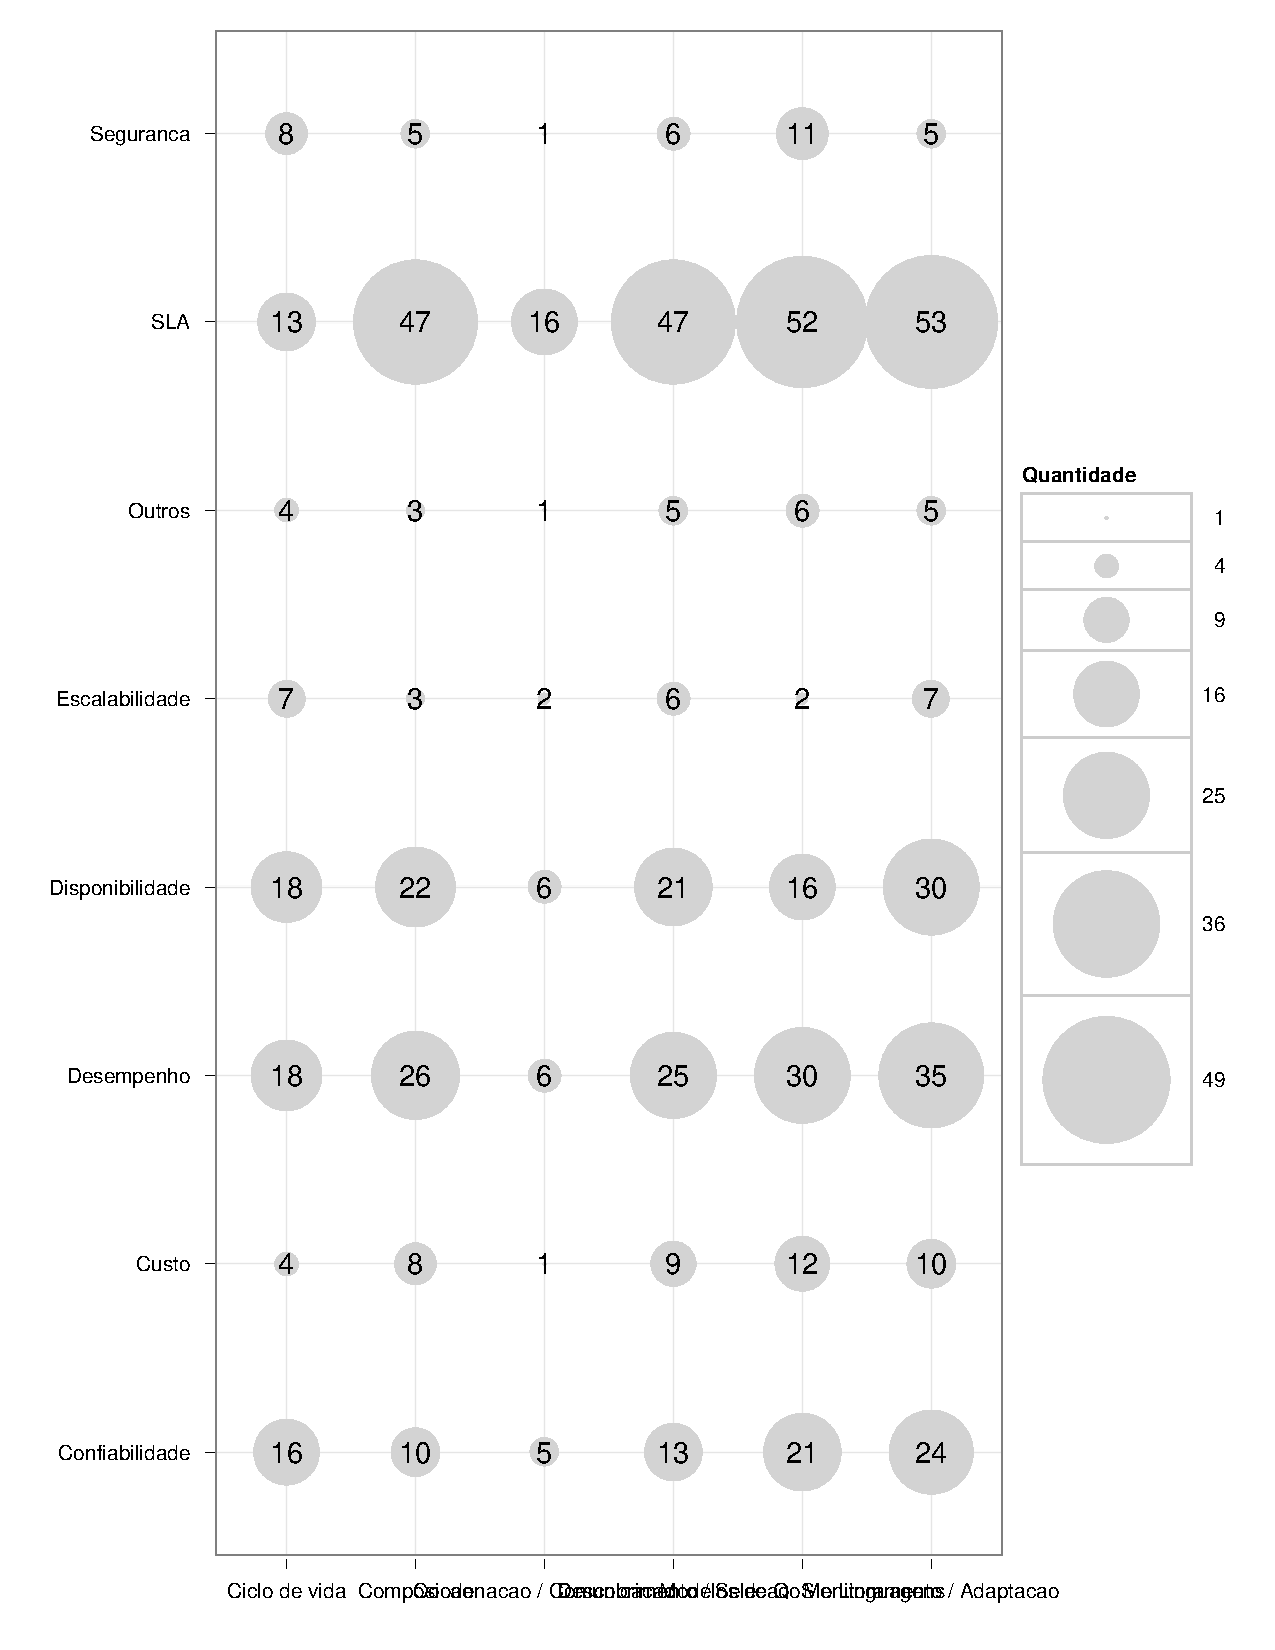
\includegraphics[scale=0.4]{imagens/contribuicaoContexto.pdf}
\caption{\emph{Bubble plot} com a distribui\c{c}\~{a}o ap\'{o}s a realiza\c{c}\~{a}o do primeiro  estudo}
\label{fig:bubbleplot-QoSSOC}
\end{figure}

O resultado desse mapeamento mostra que a maior parte dos trabalhos publicados lida com monitoramento e adapta\c{c}\~{a}o (\MonitoramentoAdaptacao), seguida de modelos de QoS \& linguagens (\ModelosdeQoSeLinguagens), descoberta \& sele\c{c}\~{a}o (\DescobrimentoSelecao),  composi\c{c}\~{a}o (\Composicao), ciclo de vida (\Ciclodevida) e finalmente coordenação com \CoodenacaoComunicacao.

Esses resultados indicam o foco dado a aspectos não funcionais, dinâmicos e que podem sofrer variações devido a concorrência e poss\'{i}veis falhas dos servi\c{c}os em tempo de execu\c{c}\~{a}o. Uma preocupa\c{c}\~{a}o que pode refletir problemas no modelo de terceirização de serviços. Uma outra observa\c{c}\~{a}o: dado que o ambiente SOC possui características próprias e diferenciadas, é natural que novas métricas de QoS tenham sido definidas ou que métricas já utilizadas tenham ganho novos significados, assim como linguagens e especificações que admitam o tratamento e negociação dos requisitos de qualidade. O resultado obtido nesse estudo para o atributo de modelos de QoS e linguagens atesta essa constatação. Nota-se também que a descoberta e seleção de serviços foi bem endereçada nas pesquisas, assim como a composição. No primeiro grupo, é considerado o descobrimento e escolha entre serviços de mesma funcionalidade, porém com diferentes níveis de QoS. O segundo abrange não somente a composição, mas também a escolha da melhor configuração de modo a atender aos níveis globais desejáveis ou necessários de QoS para um conjunto de serviços. Por fim, notou-se um número reduzido de trabalhos que abordam ciclo de vida e menos expressivo ainda com rela\c{c}\~{a}o a coordenação \& comunicação. 

\subsection{Quest\~{a}o de Pesquisa 2}
\emph{Quais atributos de qualidade são frequentemente considerados nos estudos abordados?}

Para responder a essa pergunta, olhamos a distribui\c{c}\~{a}o dos artigos no eixo de QoS, a faceta de contexto. O eixo vertical da Figura~\ref{fig:bubbleplot-QoSSOC} apresenta os resultados dessa distribui\c{c}\~{a}o. Vale ressaltar que, como cada artigo pode tratar de m\'{u}ltiplos atributos de QoS, a soma total do n\'{u}mero de artigos mapeados em cada um dos atributos n\~{a}o totalizar\'{a} o n\'{u}mero de artigos inclu\'{i}dos no mapeamento. Por exemplo, o artigo~\cite{DBLP:journals/tse/CalinescuGKMT11} lida com os atributos de disponbilidade, desempenho e confiabilidade. 

O mapa mostra que SLA (90\% dos artigos) \'{e} o que predomina, seguido de desempenho (59.2\% dos artigos), disponibilidade (49.6\% dos artigos) e confiabilidade (38\% dos artigos). Os atributos menos observados s\~{a}o custo (19.6\% dos artigos), seguran\c{c}a (16.4\% dos artigos) e escalabilidade (13.2\% dos artigos). Os atributos que n\~{a}o se enquadraram especificamente em nenhum desses foram classificados em outros (9.2\% dos artigos) como aqueles que envolvem outros atributos de qualidade como, por exemplo, \cite{6036406} que define um crit\'{e}rio de sele\c{c}\~{a}o de servi\c{c}o conforme sua reputa\c{c}\~{a}o. 

A partir desses resultados, pode-se notar que, no contexto de SOC, os termos mais relacionados a QoS s\~{a}o SLA, desempenho, disponibilidade e confiabilidade, com bastante \^{e}nfase em SLA. No entanto, observamos muitas vezes que os trabalhos mencionavam QoS sem explicitar qual atributo em particular estava em quest\~{a}o. Nesses casos, com base nas m\'{e}tricas utilizadas, classificamos como SLA por ser a op\c{c}\~{a}o mais pr\'{o}xima naquele contexto. Dessa forma, considerando essa classifica\c{c}\~{a}o do SLA como poss\'{i}vel lacuna de clareza nos trabalhos avaliados, os dados gerais nos induzem a concluir que desempenho, disponibilidade e confiabilidade s\~{a}o prioridade como atributos de QoS em SOC. No entanto, o mesmo n\~{a}o pode ser conclu\'{i}do para seguran\c{c}a, escalabilidade e custo. 
\subsection{Quest\~{a}o de Pesquisa 3}
\emph{Quais atributos de qualidade são frequentemente considerados nos estudos abordados?}

Para responder a essa pergunta, olhamos a distribui\c{c}\~{a}o dos artigos no eixo de QoS, a faceta de contexto. A Figura~\ref{Fig:bubbleplot} apresenta o diagrama ilustrando essa distribui\c{c}\~{a}o. Vale ressaltar que, como cada artigo pode tratar de m\'{u}ltiplos atributos de QoS, a soma total do n\'{u}mero de artigos mapeados em cada um dos atributos n\~{a}o totalizar\'{a} o n\'{u}mero total de artigos inclu\'{i}dos no mapeamento. Por exemplo, o artigo~\cite{DBLP:journals/tse/CalinescuGKMT11} lida com os atributos de disponbilidade, desempenho e confiabilidade. 

O mapa mostra que SLA (90\% dos artigos) \'{e} o que predomina, seguido de desempenho (59.2\% dos artigos), disponibilidade (49.6\% dos artigos) e confiabilidade (38\% dos artigos). Os atributos menos observados s\~{a}o custo (19.6\% dos artigos), seguran\c{c}a (16.4\% dos artigos) e escalabilidade (13.2\% dos artigos). Os atributos que n\~{a}o se enquadraram especificamente em nenhum desses foram classificados em outros (9.2\% dos artigos) como aqueles que envolvem outros atributos de qualidade como, por exemplo, \cite{6036406} que define um crit\'{e}rios de sele\c{c}\~{a}o de servi\c{c}o conforme sua reputa\c{c}\~{a}o. 

\subsection{Questão de Pesquisa 4}\label{sub:QP4}

\textbf{Qual o foco da contribuição de pesquisa realizada em SOC e relacionada com qualidade de serviço? }
\\[0.01in]

Com o intuito de responder a esta questão, foi feita uma avalia\c c\~{a}o da distribui\c c\~{a}o dos 
artigos em rela\c c\~{a}o ao tipo de pesquisa (conforme discutido na Se\c c\~{a}o~\ref{sec:review_method}). 
O \emph{bubble plot} na Figura~\ref{fig:bubbleplot-QoSRes}  apresenta tal distibui\c c\~{a}o, novamente sendo importante ressaltar que o n\'{u}mero total de artigos nos gr\'{a}ficos \'{e} superior ao n\'{u}mero total de artigos analisados--- uma vez que alguns artigos apresentam contribui\c c\~{o}es tanto em termos de uma nova solu\c c\~{a}o proposta quanto em termos de avalia\c c\~{a}o e/ou valida\c c\~{a}o. Por exemplo, Huang et al. prop\~{o}e um modelo estoc\'{a}stico para representar e raciocinar sobre dependabilidade em um ambiente de SOC, ao mesmo tempo que valida formalmente tal proposta por meio de provas de teoremas~\cite{huang:scc2011}.

\begin{figure*}[htb]
\centering
\includegraphics[scale=0.55]{imagens/pesquisaContexto3.pdf}
\caption{\emph{Bubble plot} com a distribui\c{c}\~{a}o envolvendo tipos de pesquisa e contexto(QoS)}
\label{fig:bubbleplot-QoSRes}
\end{figure*}

Esta investiga\c c\~{a}o revelou que 155 artigos ou 42.5\% do total apresentam, al\'{e}m de uma nova solu\c c\~{a}o relacionada \`{a} qualidade de servi\c cos em SOC, uma validação da proposta por meio de experimentos e simulações empíricas (e.g.  ~\cite{jeong:fqs2009,ardagna:jss2010,huang:scc2011,binshtok:icsoc2009}). Por outro lado, 163 artigos ou 44.8\% s\~{a}o propostas de solu\c c\~{o}es que não apresentam validações empíricas, isto é, carecem de experimentos que demonstrem a viabilidade e benefícios da(s) técnica(s) propostas. Entre esses artigos podemos citar \cite{filieri:faa2012,nascimento:splc2011,balfagih:icime2011,Clark:2009}. Finalmente, 33 artigos (9\%) foram classificados como avaliação, sendo que 10 apresentam, al\'{e}m de uma nova solu\c c\~{a}o relacionada \`{a} qualidade de servi\c cos em SOC, uma avaliação de técnicas correlatas em casos de uso reais, avaliando as limitações e benefícios das soluções existentes, e 23 artigos (6.3\%) avaliam em casos de uso reais propostas existentes 
identificando seus benefícios e limitações.

Esses n\'{u}meros revelam que a \'{a}rea de pesquisa de qualidade de servi\c co em SOC ainda est\'{a} em uma fase de amadurecimento naquilo que se refere ao uso e adoção em casos de uso reais das propostas, dada o baixo percentual dos artigos classificados como avaliação (9\%), o que indica a necessidade de mais pesquisas capazes de comparar diferentes técnicas já existentes. Também observou-se que um percentual significativo das contribui\c c\~{o}es simplesmente apresentam novas abordagens ou fazem compara\c c\~{o}es envolvendo a pr\'{o}pria t\'{e}cnica proposta (44.8\%).%--- o que refuta nossa hipótese inicial de que pesquisas relativas a QoS em SOC estejam próximas a um patamar de amadurecimento, conforme o ciclo de maturação de Redwine et al. \cite{redwine:icse1985}.




\section{Amea\c cas a validade}

As poss\'{i}veis amea\c as a aos 
resultados dessa pesquisa, bem como a generaliza\c c\~{a} dos mesmos, 
s\~{a}o descritas nessa se\c c\~{a}o, conforme a 
classifica\c c\~{a}o apresentada em~\cite{leedy1980practical}. 

\noindent
\emph{A Validade de constru\c c\~{a}o} est\'{a} relacionada
\`{a}s decis\~{o}es operacionais que foram tomadas, durante o
planejamento do estudo, com o intuito de responder \`{a}s quest\~{o}es de
pesquisa. As principais constru\c{c}\~{o}es do nosso estudo est\~{a}o em \textbf{definir os conceitos de ``QoS em SOC''}, definir o per\'{i}odo de publica\c{c}\~{o}es significativa para o estudo e \textbf{o mapeamento do estudo em si}. Como nosso objetivo \'{e} identificar tend\^{e}ncias de pesquisa na \'{a}rea de QoS em SOC, o fato de n\~{a}o termos considerado trabalhos publicados ap\'{o}s Dezembro de 2011 pode representar uma amea\c ca aos nossos resultados. Por outro lado, consideramos que trabalhos publicados entre Janeiro de 2009 e Dezembro de 2011 permitem o estabelecimento de uma tend\^{e}ncia, uma vez que n\~{a}o observamos varia\c c\~{o}es significativas durante esses anos em rela\c c\~{a}o \`{a}s facetas investigadas, em particular ao tipo de
contribui\c c\~{a}o (\textbf{Genaína: não entendi bem a partir de ``UMA VEZ QUE''... acho que não está refletindo bem o porquê}. Tirar? Refinar?). Al\'{e}m disso, consideramos que uma avalia\c c\~{a}o parcial do ano corrente (2012) poderia levar a avalia\c{c}\~{o}es
inconclusivas. Finalmente, com a infraestrutura que disponibilizamos para a realiza\c
c\~{a}o de mapeamentos sistem\'{a}ticos de estudos, podemos tanto estender 
essa investiga\c c\~{a}o em um trabalho futuro quanto convidarmos outros 
pesquisadores para replicar tal avalia\c c\~{a}o. \textbf{Gena\'{i}na: Para realizar nosso estudos seguimos as diretrizes de ref\^{e}ncia de Kitchenham~\cite{kitchenham:techReport2007} para definir as quest\~{o}es de pesquisa, crit\'{e}rio de busca e protocolo do estudo.}

\noindent
\emph{A Validade interna}
Estabelece a rela\c{c}\~{a}o causal garantindo que certas condi\c{c}\~{o}es levem de fato a outras condi\c{c}\~{o}es. Em particular, a ameaça nesse sentido consiste na seleção incompleta ou inadequada das contribuições ou a tendenciosidade da visão individual de cada pesquisador envolvido... \textbf{Genaína: A seleção correta pode ser percebida tanto definição adequada do protocolo na Seção~\ref{sec:review_method} quanto por resultados conclusivos como aqueles apresentados por principais grupos na Se\c{c}\~{a}o ~\ref{sec:QP3}}.

\noindent
\emph{A Validade externa} est\'{a} relacionada com a possibilidade de
generaliza\c c\~{a}o do nosso estudo. Esse \'{e} um aspecto muito
importante que est\'{a} relacionado ao escopo do nosso estudo, que tem
como objetivo entender a pesquisa realizada em QoS / SOC. Por outro
lado, o termo QoS \'{e} bastante amplo, sendo invi\'{a}vel realizar
um estudo compreensivo sobre todos os atributos de qualidade
relacionados a SOC (seguran\c ca, performance, toler\^{a}ncia a falhas
etc.). Nesse sentido, e conforme discutido na se\c c\~{a}o~\ref{sec:review_method}, a
nossa \texttt{string} de busca se restringiu aos termos \emph{quality
  of services}, \emph{quality of service} e \emph{QOS}. Tais termos
deveriam aparecer em algum campo de metadados de um artigo (como
t\'{i}tulo, rsumo ou palavras-chave) para que o mesmo fosse recuperado pelo
\emph{crawler} desenvolvido. Ou seja, n\~{a}o generalizamos nossos
resultados para pesquisas desenvolvidas em uma \'{a}rea espec\'{i}fica de
QOS, mas sim para a \'{a}rea de QOS de forma mais gen\'{e}rica. Como
trabalho futuro, temos
o interesse de reproduzir mapeamentos sistem\'{a}ticos de estudo para
algumas \'{a}reas espec\'{i}ficas de QOS (tratamento de exce\c
c\~{o}es, seguran\c ca etc). 

\noindent
\emph{A confiabilidade} est\'{a} relacionada ao grau de objetividade de
um estudo, em que uma poss\'{i}vel replica\c c\~{a}o levaria a
resultados parecidos. \'{E} importante destacar que um estudo abrangente como este,
envolvendo cinco pesquisadores, leva a algum risco nesse sentido,
uma vez que a classifica\c c\~{a}o dos artigos envolve certo grau
subjetividade--- cada pesquisador, com base na leitura de algumas
se\c c\~{o}es de um artigo, precisa caracterizar o trabalho de acordo
com as facetas do estudo. Com o intuito de minimizar tal subjetividade,
algumas reuni\~{o}es objetivaram esclarecer as facetas do estudo,
enquanto que outras serviram para realizar avalia\c c\~{o}es em
pares. Finalmente, foram feitas discuss\~{o}es entre os autores deste
trabalho sempre que a an\'{a}lise de um artigo resultava em d\'{u}vidas
quanto sua classifica\c c\~{a}o. 

\section{Conclus\~{a}o e Trabalho Futuro}\label{sec:conclusao}

Esse artigo apresenta um mapeamento sistem\'{a}tico na \'{a}rea 
de \emph{Qualidade de Servi\c co} em \emph{Computa\c c\~{a}o Orientada a Servi\c cos}, visando identificar 
(a) o tipo e maturidade da pesquisa realizada; (b) os atributos de qualidade e componentes de SOC considerados; e (c) os principais grupos interessados no tema. Os dados obtidos tra\c{c}aram um panorama da pesquisa relacionada, servindo de insumo e orientação para o aprofundamento de novas pesquisas nas diferentes tópicos envolvidos e identificando aspectos importantes da maturidade da pesquisa dentro do período avaliado. Consideramos que a definição dos tópicos mais relevantes de QoS em SOC como uma faceta de classificação, constituiu também uma das contribuições do artigo ao final do estudo. Além disso, determinou-se quais aspectos de qualidade tiveram maior destaque entre as pesquisas avaliadas, evidenciando não só o interesse dos pesquisadores, mas também possíveis lacunas de pesquisa em termos de QoS em ambientes orientados a serviços. Por fim, foi possível a identificação de grupos de pesquisa mais ativos na área em questão, o que possibilita o aprofundamento dos resultados por meio de técnicas de \textit{snow-balling} e também fornece um ponto de partida para revisões sistemáticas de literatura.

Como trabalho futuro, consideramos aprimorar a ferramenta de mapeamento criada para viabilizar esse estudo de modo a permitir melhor usabilidade com as bibliotecas digitais e viabilizar o uso de técnicas como \emph{snowball}. Quanto ao mapeamento sistem\'{a}tico em si, pretendemos utilizar a base de dados aceita para a realiza\c{c}\~{a}o de uma revis\~{a}o sistem\'{a}tica da literatura (\emph{Systematic Literature Review}) com vistas a uma avalia\c{c}\~{a}o mais aprofundada dos trabalhos avaliados, como por exemplo, seus benef\'{i}cios e limita\c{c}\~{o}es, assim como suas contribui\c{c}\~{o}es relativas \`{a} arquitetura de software.

%Entre as principais considera\c c\~{o}es, podemos destacar que a pesquisa envolvendo QoS e SOC parece estar nos est\'{a}gios iniciais, uma vez que boa parte do esfor\c co est\'{a} relacionada a proposi\c c\~{a}o de novas t\'{e}cnicas--- sendo que poucos trabalhos buscam coletar evid\^{e}ncias da efic\'{a}cia de propostas existentes.  Al\'{e}m disso,  

%Finalmente, \'{e} importante observar que alguns estudos apontam para uma promissora intera\c{c}\~{a}o entre nuvens computacionais e SOC~\cite{10.1109/MIC.2010.147}, onde a maior intersec\c{c}\~{a}o entre ambas seria no contexto de \emph{software} como serviço. Para atender a essa nova atua\c{c}\~{a}o para SOC, acreditamos que muitos pontos levantados nesse mapeamento podem ser relevantes para o modelo de computa\c{c}\~{a}o em larga escala proposto pela computação em nuvens, o que poderá ser verificado num trabalho futuro.


\bibliographystyle{sbc}
\bibliography{sbc-template}

\end{document}
